\documentclass{article}
\usepackage[slovene]{babel}
\pdfpagewidth=8.5in
\pdfpageheight=11in
\usepackage{ijcai19}
\usepackage{listings}
% Use the postscript times font!
\usepackage{times}
\usepackage{soul}
\usepackage{url}
\usepackage[hidelinks]{hyperref}
\usepackage[utf8]{inputenc}
\usepackage[small]{caption}
\usepackage{graphicx}
\usepackage{amsmath}
\usepackage{multirow}
\usepackage{longtable}
\usepackage{geometry}
\usepackage{array}
\usepackage{booktabs}
\usepackage{makecell}
\usepackage{subcaption}
\urlstyle{same}

\title{Tretja domača naloga}

\author{
Matej Klančar (63200136)
}

\begin{document}
\maketitle
\vspace{-1.5cm}
\section{Uvod}
V tem poročilu obravnavamo problem matematičnega nihala, katerega gibanje opisuje nelinearna 
diferencialna enačba drugega reda. Za majhne odklone se ta enačba pogosto poenostavi v model 
harmoničnega nihala, katerega perioda je za razliko od pravega nihala neodvisna od amplitude.

Osrednji cilj naloge je raziskati razlike med tema dvema modeloma. Z uporabo numeričnih metod v 
programskem jeziku Julia rešujemo sistem diferencialnih enačb prvega reda. 

V poročilu najprej predstavimo teoretično ozadje problema, 
sledi opis implementacije numerične rešitve, na koncu pa so zbrani in interpretirani rezultati
z grafičnimi prikazi.
\section{Opis problema}

Naloga obravnava nedušeno nihanje matematičnega nihala. Kotni odmik 
nihala $\theta(t)$ v odvisnosti od časa $t$ je opisan z nelinearno diferencialno 
enačbo drugega reda:
\begin{equation}
\ddot{\theta}(t) + \frac{g}{l} \sin(\theta(t)) = 0
\label{eq:nelinearna}
\end{equation}
kjer je $g$ težni pospešek in $l$ dolžina vrvice nihala. Začetni pogoji
 so podani kot $\theta(0) = \theta_0$ in $\dot{\theta}(0) = \dot{\theta}_0$.

\subsection{Prevedba na sistem prvega reda}
Za numerično reševanje je potrebno enačbo \eqref{eq:nelinearna} prevesti na sistem dveh diferencialnih enačb prvega reda. 
To storimo z uvedbo novih spremenljivk:
\begin{itemize}
    \item $y_1(t) = \theta(t)$ (kotni odmik)
    \item $y_2(t) = \dot{\theta}(t)$ (kotna hitrost)
\end{itemize}
Z odvajanjem teh spremenljivk po času dobimo sistem:
\begin{align}
\dot{y}_1(t) &= y_2(t) \\
\dot{y}_2(t) &= -\frac{g}{l} \sin(y_1(t))
\end{align}
Ta sistem je primeren vhod za metode, ki diferencialne enačbe rešujejo z numeričnimi metodami.
V tej nalogi uporabimo metodo DOPRI5 (Dormand-Prince 5).

\subsection{Harmonična aproksimacija}
Za majhne začetne odklone ($\theta_0 \ll 1$) lahko funkcijo $\sin(\theta)$ aproksimiramo z 
$\sin(\theta) \approx \theta$. S tem poenostavimo enačbo \ref{eq:nelinearna} v enačbo za harmonično nihalo:
\begin{equation}
\ddot{\theta}(t) + \frac{g}{l} \theta(t) = 0
\label{eq:linearna}
\end{equation}
Analitična rešitev te enačbe (ob predpostavki $\dot{\theta}(0) = 0$) je:
\begin{equation}
\theta(t) = \theta_0 \cos(\omega t), \quad \text{kjer je } \omega = \sqrt{\frac{g}{l}}
\end{equation}
Perioda nihanja pri harmonični aproksimaciji je konstantna in enaka $T = 2\pi/\omega$. Je neodvisna 
od začetne amplitude $\theta_0$.

\subsection{Cilji naloge}
\begin{enumerate}
    \item Želimo implementirati funkcijo, ki numerično reši sistem diferencialnih enačb za 
    matematično nihalo.
    \item Želimo primerjati numerično rešitev nelinearnega matematičnega nihala 
    z analitično rešitvijo harmoničnega nihala.
    \item Želimo analizirati in grafično prikazati, kako je nihajni čas 
    matematičnega nihala odvisen od njegove začetne energije, ki jo določa začetni kot $\theta_0$.
\end{enumerate}


\section{Implementacija}

Rešitev je bila implementirana v programskem jeziku Julia z uporabo knjižnic za
numerično reševanje diferencialnih enačb in za vizualizacijo rezultatov.

\subsection{Definicija sistema}
Sistem diferencialnih enačb prvega reda je bil definiran v funkciji, ki za reševalnik
izračuna odvode stanj. Funkcija kot vhod prejme trenutno stanje (kot in kotna hitrost),
parametre (težni pospešek in dolžina) ter čas, kot izhod pa vrne vektor odvodov. Prva
komponenta izhodnega vektorja je sprememba kota (enaka kotni hitrosti), druga pa sprememba
kotne hitrosti (enaka kotnemu pospešku, izračunanemu iz enačbe gibanja).

\subsection{Reševanje diferencialne enačbe}
Za reševanje problema je bila implementirana posebna funkcija, ki združi vse potrebne
komponente. Najprej definira problem z združitvijo funkcije sistema, začetnih pogojev,
časovnega intervala simulacije in fizikalnih parametrov. Ta problem se nato posreduje
reševalniku, ki temelji na eksplicitni metodi Runge-Kutta Dormand-Prince 5. reda (DOPRI5).
Ta metoda je primerna za širok spekter problemov in je znana po svoji natančnosti in
učinkovitosti. Funkcija na koncu vrne časovne točke in izračunane kotne odklone.

\subsection{Analiza in vizualizacija}
Implementirane so bile tri pomožne funkcije za analizo in prikaz rezultatov:
\begin{itemize}
    \item \textbf{Funkcija za oceno periode nihanja:} Ta funkcija oceni periodo tako,
    da iz časovne vrste rešitve poišče čas, ko nihalo prvič prečka ravnovesno
    ego ($\theta=0$). Ta čas predstavlja četrtino periode ($T/4$), zato ga pomnožimo
    s 4, da dobimo oceno za celotno periodo.

    \item \textbf{Funkcija za primerjavo modelov:} Za poljuben začetni kot izračuna rešitev
    za nelinearni model in za harmonično aproksimacijo. Obe rešitvi nato izriše na skupni graf,
    kar omogoča neposredno vizualno primerjavo odmikov in period.

    \item \textbf{Funkcija za risanje odvisnosti periode:} Ta funkcija sistematično razišče
    odvisnost periode od energije. V zanki iterira čez vnaprej določeno območje začetnih kotov,
    za vsakega reši enačbo nihala, oceni periodo in na koncu izriše graf,
    ki prikazuje, kako perioda narašča z večanjem začetnega kota.
\end{itemize}

\section{Primerjava rezultatov}

Na podlagi implementacije smo generirali grafe, ki prikazujejo ključne lastnosti matematičnega nihala.

\subsection{Odvisnost periode od začetnega kota}
Najprej smo analizirali, kako se perioda nihanja spreminja z začetnim kotom. Za harmonično 
nihalo bi pričakovali konstantno periodo $T = 2\pi\sqrt{l/g} \approx 2.006$s (ob $l = 1$m). 
Rezultati za nelinearno matematično nihalo so prikazani na sliki \ref{fig:perioda}.

\begin{figure}[h!]
    \centering
    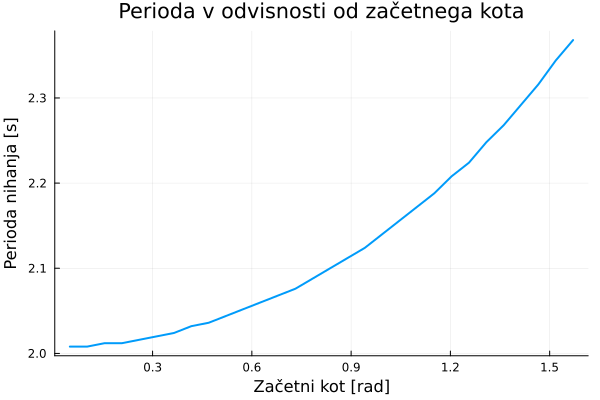
\includegraphics[width=0.8\textwidth]{../slike/perioda_vs_kot.png}
    \caption{Odvisnost periode nihanja od začetnega kota za matematično nihalo. Pričakovana perioda 
    za harmonično nihalo je približno 2.0 s.}
    \label{fig:perioda}
\end{figure}

Iz grafa je jasno razvidno, da perioda matematičnega nihala ni konstantna, temveč narašča z večanjem 
začetnega kota (in s tem energije nihala). Pri majhnih kotih je perioda blizu 2s, kot pri harmoničnem nihalu. 
Z večanjem amplitude pa postaja odstopanje vse večje.

\subsection{Primerjava z harmonično aproksimacijo}
Na slikah v figuri \ref{fig:primerjave} je prikazana primerjava časovnega poteka nihanja med nelinearnim 
modelom (polna črta) in harmonično aproksimacijo (črtkana črta) za različne začetne kote, od $22.5^\circ$ do $90^\circ$.

\begin{figure}[h!]
    \centering
    \begin{subfigure}[b]{0.49\textwidth}
        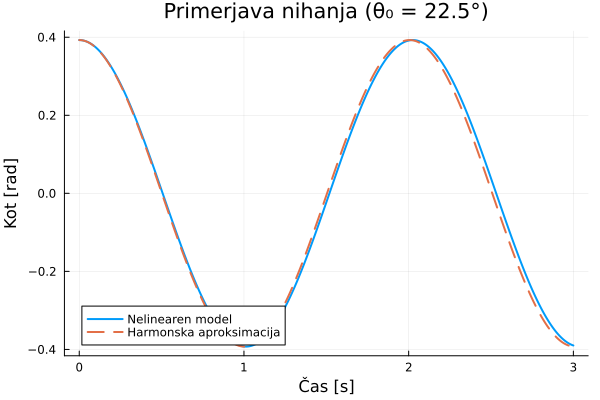
\includegraphics[width=\textwidth]{../slike/primerjava_0.39.png}
        \caption{$\theta_0 = 22.5^\circ$}
        \label{fig:comp22}
    \end{subfigure}
    \hfill
    \begin{subfigure}[b]{0.49\textwidth}
        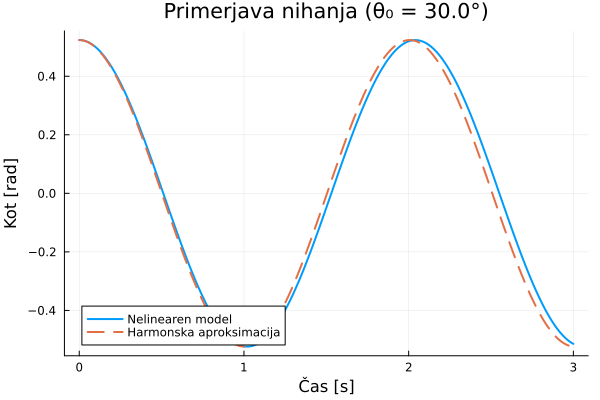
\includegraphics[width=\textwidth]{../slike/primerjava_0.52.png}
        \caption{$\theta_0 = 30.0^\circ$}
        \label{fig:comp30}
    \end{subfigure}
    
    \vspace{1cm} % Dodaten prostor med vrsticami
    
    \begin{subfigure}[b]{0.49\textwidth}
        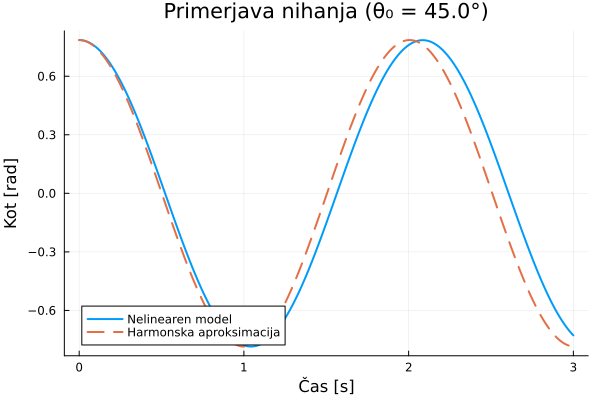
\includegraphics[width=\textwidth]{../slike/primerjava_0.79.png}
        \caption{$\theta_0 = 45.0^\circ$}
        \label{fig:comp45}
    \end{subfigure}
    \hfill
    \begin{subfigure}[b]{0.49\textwidth}
        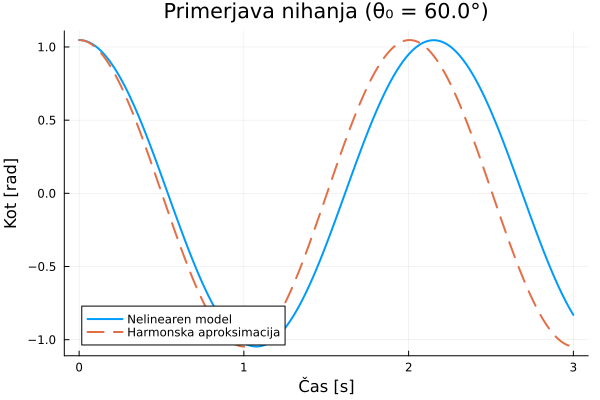
\includegraphics[width=\textwidth]{../slike/primerjava_1.05.png}
        \caption{$\theta_0 = 60.0^\circ$}
        \label{fig:comp60}
    \end{subfigure}
    
    \vspace{1cm}
    
    \begin{subfigure}[b]{0.49\textwidth}
        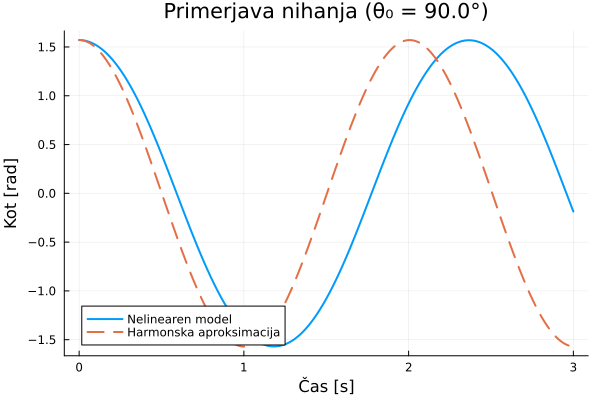
\includegraphics[width=\textwidth]{../slike/primerjava_1.57.png}
        \caption{$\theta_0 = 90.0^\circ$}
        \label{fig:comp90}
    \end{subfigure}
    
    \caption{Primerjava rešitve nelinearnega modela (polna črta) in harmonične aproksimacije (črtkana črta) 
    za različne začetne kote.}
    \label{fig:primerjave}
\end{figure}

Opazimo lahko naslednje:
\begin{itemize}
    \item Pri manjših kotih (sliki \ref{fig:comp22} in \ref{fig:comp30}) je ujemanje med modeloma zelo dobro. 
    Harmonična aproksimacija je ustrezna, čeprav se že po nekaj nihajih pojavi majhen fazni zamik.
    \item Z večanjem kota (sliki \ref{fig:comp45} in \ref{fig:comp60}) postanejo razlike očitne. Perioda 
    nelinearnega nihala je vidno daljša, kar povzroči, da zaostaja za harmonično aproksimacijo.
    \item Pri velikem kotu $90^\circ$ (slika \ref{fig:comp90}) je harmonična aproksimacija povsem nezadostna. 
    Perioda matematičnega nihala je bistveno daljša, kar potrjuje opažanja iz slike \ref{fig:perioda}.
\end{itemize}
Rezultati jasno kažejo meje veljavnosti linearizacije in potrjujejo, da je nelinearni člen $\sin(\theta)$ 
ključen za pravilen opis nihanja pri večjih amplitudah.


\end{document}